\documentclass[12pt,fancy]{cours}
\Chapit{2}{4}
\begin{document}
\begin{center}
  \Large
  \color{structurecolor}
  \textsc{Préparation aux écrits de Physique}
\end{center}

% --------------------------------------------------------------
%                         Start here
% --------------------------------------------------------------
%
% \lhead{PC Théophile Gautier}
% %\chead{L.Villa}
% \rhead{Révision des écrits}

\section{Préparation aux épreuves}

\subsection{Stratégie de préparation}

\parag{Calendrier}
Davantage d'information sur le site du concours : 
\begin{center}
  \href{https://www.scei-concours.fr/calendrier.php}{https://www.scei-concours.fr/calendrier.php}.
\end{center}
Vous trouverez également un ensemble de plaquettes explicatives sur Cahier de prépa :
\begin{center}
  \href{https://cahier-de-prepa.fr/pc-theo/docs?rep=116}{https://cahier-de-prepa.fr/pc-theo/docs?rep=116}.
\end{center}

\begin{figure}[H]
  \centering
  
\includegraphics[width=\textwidth]{calendrier_ecrits_scei_2026.jpg}
  \caption{Calendrier des épreuves écrites en 2026.}
  \label{fig:}
\end{figure}
\parag{Organisation des révisions}
Avant les écrits CCINP-E3A, vous disposez de presque \imp{15 jours} pour vos révisions.  Cela peut paraître peu vu la quantité de choses à revoir, mais...
\begin{itemize}
\item \imp{Révision} n'est pas apprentissage.


Le plus gros du travail est derrière vous, quoiqu'il arrive vous ne rattraperez pas deux ans de travail en deux semaines.
\item \imp{Efficacité} prime sur quantité.

Il est préférable de travailler 8h efficacement que 12h inefficacement. Pour réviser efficacement : reprendre les fiches de synthèse et non le cours entier, vérifier que vous savez restituer les formules et les démonstrations classiques, refaire les exercices classiques de TD en identifiant le squelette de l'exercice et les questions type.


\item La \imp{forme physique et mentale} est cruciale.

Il faut arriver le jour J en bonne forme physique et mentale : faites du sport les jours précédents, ne pas tomber malade, mangez équilibré, dormez suffisamment, arrivez avec un bon état d'esprit, réduisez au maximum les sources de stress, comme le logement, les transports, les repas,etc.

\end{itemize}
\medskip

Partons sur une base de travail de \imp{8h par jour}  : 4h le matin, 4h l'après-midi, sieste ou pause recommandée entre les deux. Je vous propose le \imp{découpage horaire} suivant selon vos objectifs aux concours CCINP et E3A.
\begin{enumerate}
  \item 
  CCINP option \imp{physique} :
  $$\fbox{
  % \begin{center}
    Physique : 2h15,~\hfill
    Maths : 2h15,~\hfill
    Chimie : 1h30,~\hfill
    Info : 1h,~\hfill
    Français : 30 min,~\hfill
    Anglais : 30 min.
  % \end{center}
  }$$
  \item 
  CCINP option \imp{chimie} :
  $$\fbox{
  % \begin{center}
    Chimie : 2h15,~\hfill
    Maths : 2h15,~\hfill
    Physique : 1h30,~\hfill
    Info : 1h,~\hfill
    Français : 30 min,~\hfill
    Anglais : 30 min.
  % \end{center}
  }$$
\end{enumerate}


 \parag{Pendant l'épreuve} Les règles fondamentales d'une bonne rédaction.
 \begin{enumerate}
 \item Rendre une copie \imp{soignée} :
 
 résultats importants encadrés, lois et hypothèses soulignées, schémas clairs et légendés, démonstration structurée en paragraphes, pas de ratures, etc.
 
 \item Vérifier la \imp{cohérence} des résultats :
 
 vérifier que les résultats sont homogènes, qu'un vecteur est bien égal à un vecteur et un scalaire à un scalaire, vérifier la cohérence d'une application numérique, etc.
 \end{enumerate}
 Dans les dernières minutes d'une épreuve, relire ce que vous avez fait pour respecter ces critères. Il est essentiel de faire bonne impression au correcteur. Faites aussi attention à l'orthographe !


\subsection{Concours CCINP et E3A-Polytech}
\parag{Généralités}
  Pour les écoles spécifiques vous pouvez consulter le tableau ci-dessous.
Les banques CCINP et E3A-Polytech sont très similaires, et les épreuves écrites sont partiellement mutualisées. Cependant, les épreuves scientifiques principales sont spécifiques à chaque banque, comme indiqué sur le \Tab{coefficients} ci-dessous.  Pour les écoles spécifiques de chaque banque, consulter la \Fig{coefficients}.

\def\note{{\color{JoliRouge}\textsuperscript{*}}}
\def\nnote{{\color{JoliBleu}\textsuperscript{**}}}
\def\Note{{\color{JoliRouge}{\large {$\star$}}}}
\def\Nnote{{\color{JoliBleu}{\large {$\star\star$}}}}

\begin{table}[H]
  \centering
  \begin{tabular}{|l|l|l|l|l|l|}

    \hline
    Type d'épreuve & Épreuve & Durée & Coefficient & Particularité\\
    \hline
    \multirow{4}{*}{\textbf{Commune}} & Français & 4h & 9  & \\
    & Anglais & 3h & 4 & \\ 
    & Informatique & 3h & 6 & \\ 
    & Modélisation & 4h & 7 & \\
    \hline
    \multirow{3}{*}{\textbf{Spécifique CCINP}} & Maths & 4h & 12 & Sans calculatrice \\
     & Chimie & 4h & 13\note ou 7\nnote & Avec calculatrice\\
    & Physique & 4h & 7\note ou 13\nnote & Avec calculatrice\\
    \hline
    \multirow{2}{*}{\textbf{Spécifique E3A}} & Maths & 4h & & Sans calculatrice\\
    & Physique-Chimie & 4h & & Sans calculatrice\\
    \hline
  \end{tabular}
  \caption{Répartition des épreuves et coefficients pour les concours CCINP et E3A.  \\
  \small{\note CCINP option chimie, \nnote CCINP option physique.}}\
  \label{tab:coefficients}
\end{table}

% \parag{Coefficients}
% Pour le français, vous avez normalement déjà fourni le travail pour l'écrit pendant l'année. Attention à ne \imp{pas négliger} les matières littéraires, le coefficient cumulé de l'anglais et du français étant proche de celui des maths. Les \imp{coefficients} sont les suivants. 

% \begin{enumerate}
%   \item  CCINP option \imp{Physique} :
%   $$\fbox{
%   % \begin{center}
%     Physique : 13,~\hfill
%     Maths : 12,~\hfill
%     Chimie : 7,~\hfill
%     Modélisation : 7,~\hfill
%     Informatique : 6,~\hfill
%     Français : 9,~\hfill
%     Anglais : 4.
%   % \end{center}
%   }$$
%   \item CCINP option \imp{Chimie} :
%     $$\fbox{
%   % \begin{center}
%     Chimie : 13,~\hfill Maths : 12,~\hfill Physique : 7, ~\hfill Modélisation : 7, ~\hfill Informatique : 6,~\hfill Français : 9,~\hfill Anglais : 4.
%   % \end{center}
%   }$$
% \end{enumerate}
\begin{figure}[H]
  \centering
  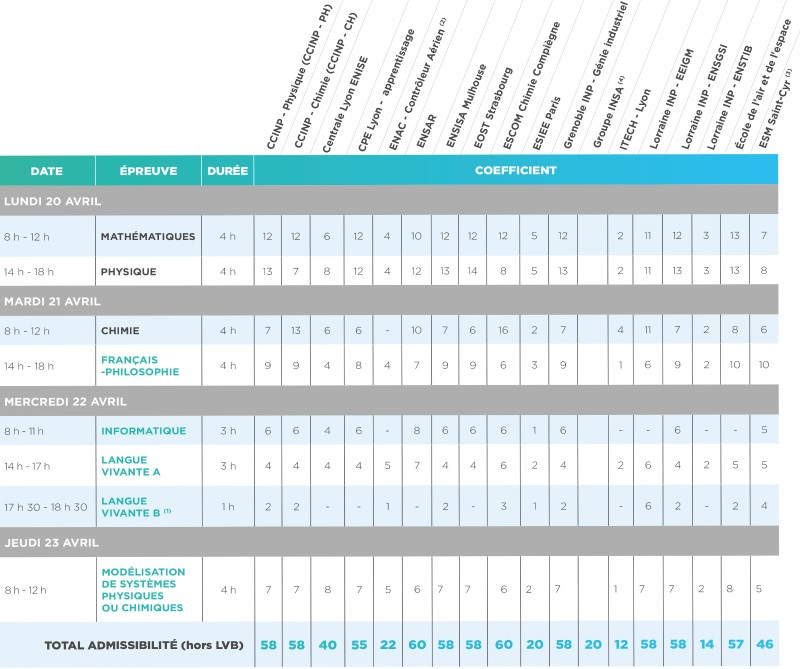
\includegraphics[width=\textwidth]{coeffitients_PC.jpg}
  \caption{Coefficients pour les écoles spécifiques du concours CCINP.}
  \label{fig:coefficients}
\end{figure}

\parag{Épreuve de Physique CCINP} Voici les consignes officielles.

«\emph{
  Utiliser uniquement un stylo noir ou bleu foncé non effaçable pour la rédaction de votre composition ; d’autres
couleurs, excepté le vert, bleu clair ou turquoise, peuvent être utilisées, mais exclusivement pour les schémas
et la mise en évidence des résultats.
 Ne pas utiliser de correcteur.
 Écrire le mot FIN à la fin de votre composition
}»

\parag{Épreuve de Physique E3A-Polytech} Voici les consignes officielles.

% \begin{center}
  «\emph{
  L’épreuve de « Physique – Chimie » spécifique à la banque e3a-Polytech est d’une durée totale de 4 heures. Elle est réalisée sans calculatrice.}

  \emph{
Elle comporte deux parties indépendantes : une partie Physique et une partie Chimie. Les deux parties ont un poids équivalent dans la note finale attribuée à l’épreuve.
La partie Physique est un problème de difficulté graduée, portant sur les diverses parties du programme de physique de PCSI/PC. L’épreuve s’intéresse principalement à un phénomène physique et elle peut mettre l’accent sur la mesure de grandeurs. Elle a pour objectif d’évaluer des connaissances en physique, à la fois par la résolution de problèmes concrets et par leur mise en équation.}

\emph{
La partie Chimie comporte un ou deux problèmes (dont l’un de chimie organique), de difficulté graduée, portant sur les diverses parties du programme de PCSI/PC. L’épreuve est focalisée sur un composé chimique, un phénomène ou un processus industriel. La partie inorganique et la partie organique sont de poids comparables. La partie organique met l’accent sur l’utilisation de données spectroscopiques. Cette épreuve a pour objectif d’évaluer la capacité du candidat à raisonner, à prévoir et à transposer ses connaissances dans des situations nouvelles ou sur des composés similaires à ceux étudiés en cours.
}

\emph{
Une rédaction soignée et des explications claires sont attendues. Le barème valorise les copies où les parties abordées sont traitées de manière complète et cohérente.}
  »
% \end{center}

\subsection{Concours Centrale-Supélec}

\parag{Généralités}

\begin{table}[H]
  \centering
  \begin{tabular}{|l|l|l|l|l|l|}
    \hline
    Épreuve & Durée & Coefficient & Particularité\\
    \hline
    Français & 4h & 17  & \\
    Anglais & 3h & 11 & \\ 
    Mathématiques 1 & 4h & 15 & Sans calculatrice \\
    Mathématiques 2 & 4h & 15 & Sans calculatrice \\
    Physique 1 & 4h & 14 & Avec calculatrice \\
    Physique 2 & 4h & 14 & Avec calculatrice \\
    Chimie & 4h & 14 & Avec calculatrice \\
    \hline
  \end{tabular}
  \caption{Répartition des épreuves et coefficients pour le concours Centrale-Supélec.}
  \label{tab:coefficients_CCS}
\end{table}

\parag{Épreuve de Physique Centrale-Supélec} Voici les consignes officielles.
«\emph{
  L’épreuve de Physique du concours Centrale-Supélec est d’une durée totale de 8 heures. Elle comporte deux parties indépendantes : une partie Physique 1 et une partie Physique 2. La partie Physique 1 est réalisée sans calculatrice, tandis que la partie Physique 2 est réalisée avec calculatrice.}

\section{Programme de révisions}


\subsection{Outils mathématiques}
\begin{liste}
  \item Géométrie :  Théorème de Thalès (lentilles minces et rayons lumineux), théorème de Pythagore (norme d'un vecteur). Périmètre d'un cercle ($2\pi r$), surface du disque $(\pi r^2$), aire de la sphère ($4\pi r^2$), volume de la boule $(\frac{4}{3}\pi r^3)$ et du cylindre $(\pi r^2 h)$.
  \item Équation différentielle :

\begin{tabular}{ll}
 ordre 1 : & $\dd{f}{t} + \frac{f}{\tau} = 0$ (solution $f(t) = A e^{-t/\tau}$) \\
 oscillateur harmonique : & $\ddd{f}{t} + \omega_0^2 f = 0$ (solution $f(t) = A \cos(\omega_0 t) +  B \sin(\omega_0 t)$) \\
 oscillateur harmonique amorti : & $\ddd{f}{t} + \frac{\omega_0}{Q} \dd{f}{t}+ \omega_0^2 f = 0$.
\end{tabular}

  \item Développements limités à l'ordre 2 :  $(1+x)^\alpha$, $\cos(x)$, $\sin(x)$, $\ln(1+x)$.
  \item Opérateurs vectoriels : $\grad f$, $\dive \Vec{v}$, $\rot \Vec{v}$.
  % (électromagnétisme et mécanique des fluides).
\end{liste}

% Projection d'un vecteur sur une base. Produit scalaire et produit vectoriel.  Expression du gradient, de la divergence et du rotationnel en cartésiennes à partir de $\vec{\nabla}$. Théorème de Stokes et de Green-Ostrogradski.


\subsection{L'essentiel du programme de PCSI}
Je vous propose ci-dessous un programme de révision minimal décomposé par année : PCSI puis PC, par thème, et par niveau de connaissance :
\begin{enumerate}
  \item[\Note] Connaissances de base.
  \item[\Nnote] {\small\emph{Connaissances d'approfondissement}.}
\end{enumerate}
Si vous n'êtes pas dans le \imp{premier tiers} de classe,concentrez-vous sur les connaissances de base.

\begin{enumerate}
\medskip
\item \textsc{Électrocinétique}.
\item[\Note] Loi des nœuds et des mailles, diviseur de tension, impédances $\underline{Z}$ pour $R,$ $L$ et $C$, association série et parallèle, filtres RC passe-bas et passe-haut, diagramme de Bode.
{\small
\item[\Nnote] \emph{Amplificateur opérationnel (régime linéaire et saturé). Loi des nœuds en terme de potentiel. Diviseur de courant. RLC-série: régimes et résonances en fonction du facteur de qualité.}
}
\medskip
\item \textsc{Mécanique}.
\item[\Note] Référentiel galiléen. Lois de Newton. Forces et énergie potentielle : tension du ressort, poids, force de Lorentz. Chute libre, oscillation d'un système masse-ressort. Forces centrales, lois de Kepler, mouvement circulaire uniforme. Théorèmes énergétiques (cinétique et mécanique).


{\small
\item[\Nnote] \emph{Coordonnées cylindriques et expression de $\vec{v}$ et $\vec{a}$.  Théorème du moment cinétique, moment d'une force. Mouvement d'une particule dans un champ $(\vec{E},\vec{B})$. Satellites géostationnaires, vitesse de libération, étude énergétique pour un mouvement elliptique à partir de l'énergie potentielle effective. Translation et rotation d'un solide autour d'un axe fixe, moment d'inertie. Lois de Coulomb du frottement de glissement.}
}
\medskip
\item \textsc{Optique géométrique}.
\item[\Note] Relations de conjugaison de Descartes. Foyers objet et image. Tracé des rayons pour une lentille mince (convergente et divergente). La loupe. Système afocal et lunette astronomique, calcul du grossissement.
{\small
\item[\Nnote] \emph{Relations de conjugaison de Newton. Fibre optique. Système optique afocal. Calcul du grandissement.}
}
\medskip
\item \textsc{Thermodynamique}.
\item[\Note] Transformations élémentaires (isochore, isotherme, isobare, adiabatique, réversible). Travail des forces de pression. Premier et second principes. Loi du gaz parfait, loi de Laplace. Machines thermiques dithermes : moteur, rendement et théorème de Carnot. Transition de phase liquide-vapeur.
{\small
\item[\Nnote] \emph{Théorie cinétique des gaz. Passage du gaz parfait au gaz réel. Changements d'état du corps pur. Modèle de l'atmosphère isotherme. Poussée d'Archimède. Lois de Joule. Modèle de la phase condensée incompressible indilatable. Machines frigorifiques.}
}
\medskip
\item \textsc{Induction}.
\item[\Note] Loi de Faraday. Circuit mobile dans un champ magnétique stationnaire : rails de Laplace.  Circuit fixe dans un champ magnétique variable : auto-induction et inductance.
{\small
\item[\Nnote] \emph{Inductance mutuelle. Principe du transformateur. Étude énergétique du haut-parleur électrodynamique.}
}
\end{enumerate}

\subsection{L'essentiel du programme de PC}
Pour plus de simplicité, je présente les choses essentielles dans l'ordre des polycopiés. Vous pouvez réviser dans l'ordre que vous voulez. Il ne faut pas se contenter de lire le cours mais bien d'être actif et de \imp{refaire les calculs et raisonnements} à partir d'une feuille blanche.
\smallskip
\begin{enumerate}
\item \textsc{Mécanique du point}
\item[\Note] Loi de composition galiléenne des vitesses. Référentiels non galiléens : translation vs rotation uniforme ; forces d'inerties d'entraînement et de Coriolis. PFD en référentiel non galiléen. Différence entre pesanteur et attraction gravitationnelle.
{\small
\item[\Nnote] \emph{TMC et TEM en référentiel non galiléen. Pendule de Foucault. Force de Coriolis et mouvements atmosphériques. Déviation vers l'est. Théorie statique des marées.}
}

\medskip
\item \textsc{Thermodynamique}
\item[\Note] Bilan sur un portion de longueur $\d x$. ARQS et résistance thermique. Diffusion thermique (flux, loi de Fourier, conditions aux limites). Diffusion de particules (flux, courant, loi de Fick). Équation de diffusion et loi d'échelle ordre de grandeur $\delta \sim \sqrt{Dt}$. Corps noir, bilan radiatif, effet de serre sans atmosphère. Lire un diagramme $(T,s)$ et $(h,p)$, calculer $q$ et $w$ en lisant $\Delta h$.
{\small
\item[\Nnote] \emph{Onde thermique en régime sinusoïdal (effet de cave). Modèle microscopique probabiliste de la diffusion de particules. Loi de Stefan, loi de Wien, Effet de serre avec atmosphère. 1er et 2nd principes industriels.}
}
\medskip
\item \textsc{Mécanique des fluides}.
\item[\Note] Ligne de courant : définition ; accélération particulaire en cartésiennes ; débit volumique, débit massique, équation de conservation de la masse ; écoulements particuliers (stationnaire, incompressible, potentiel). Écoulement parfait : équation d'Euler, loi de Bernoulli et effet Venturi. Écoulement visqueux : force visqueuse surfacique $\frac{\d \Vec{F}_v}{\d S}=\eta\frac{\partial v_x}{\partial y}\vec{e}_x$ et volumique $\Vec{f}_{\!v}=\eta\Delta\vec{v}$,
équation de Navier-Stokes, nombre de Reynolds $\Re = \frac{LU\rho}{\eta}$ et interprétation ; force de traînée, coefficient de traînée fonction de $\Re$ ; écoulement de Couette plan et de Poiseuille cylindrique. Bilan de quantité de mouvement sur un système ouvert.
{\small
\item[\Nnote] \emph{Particule de fluide et échelle mésoscopique. Écoulement parfait autour d'une sphère. Tube de Pitot et vidange d'un réservoir. Notion de couche limite visqueuse. Bilan de moment cinétique et d'énergie sur un système ouvert.}
}
\medskip
\item \textsc{Optique}
\item[\Note] Modèle scalaire de la lumière : hypothèses, chemin optique, surface d'onde, théorème de Malus, intensité lumineuse, différence de marche $\delta$, ordre d'interférences $p$. Interférences lumineuses : conditions d'interférences, formule de Fresnel. Longueur de cohérence temporelle  $\ell_{\rm{c}}\sim\frac{\lambda^2}{\Delta\lambda}$ et interprétation. Trous d'Young : calcul et expression $\delta = \frac{a x}{D}$, intensité $I(x)$ et interfrange $i$. Interféromètre de Michelson (éléments de l'interféromètre). Lame d'air : franges d'égale inclinaison, expression de $\delta$, conditions d'éclairage et d'observation ; contact optique . Coin d'air : franges d'égales épaisseur, conditions d'éclairage et d'observation. Interaction lumière-matière : absorption, émission stimulée, émission spontanée. 
{\small
\item[\Nnote] \emph{Trous d'Young : translation de la source, élargissement de la source, cohérence spatiale. Interférences à $N$ ondes. Notion sur les sources lumineuses. Interférences en lumière blanche: blanc d'ordre supérieur, teintes de Newton et spectre cannelé. Lame d'air : calcul du rayon des anneaux d'égale inclinaison, calcul de $\delta$. Coin d'air : expression de $\delta$. Faisceau gaussien : waist et longueur de Rayleigh, modèle cône-cylindre.}
}
\medskip
\item \textsc{Électromagnétisme}
\item[\Note] Électrostatique : force coulombienne, énergie potentielle électrostatique $qV$, symétries et invariances de $\vec{E}$, théorème de Gauss ; fil infini, condensateur plan, dipôle électrostatique. Magnétostatique : symétries et invariances de $\vec{B}$, théorème d'Ampère ; fil infini, solénoïde infini et moment magnétique. Régime variable : équations de Maxwell locales, courant de déplacement et conservation de la charge, vecteur de Poynting $\Poy$ et équation de conservation de l'énergie, ARQS magnétique. Conducteur ohmique : définition d'un métal, loi d'Ohm, loi de Joule, résistance électrique. Induction : loi de Faraday, force de Laplace et de Lorentz.
{\small
\item[\Nnote] \emph{Analogie électrostatique -- gravitation. Lecture et interprétation d'une carte de champ. Modèle électrostatique du noyau atomique. Modèle planétaire de l'hydrogène et relation $\mc{\vec{M}}=\gamma\vec{L}$. Magnéton de Bohr et notions sur l'aimantation de la matière. Énergie stockée dans un condensateur $\frac{1}{2}CU^2=\frac{1}{2}\varepsilon_0 E^2\times V$, énergie stockée dans une bobine $\frac{1}{2}LI^2=\frac{1}{2\mu_0}B^2\times V$. Conservation du flux de $\B$. Neutralité d'un métal, modèle de Drude. Effet Hall.}
}

\medskip
\item \textsc{Physique des ondes}
\item[\Note] Corde vibrante (hypothèse et détermination de l'équation d'onde), équation de d'Alembert, loi de Hooke, types d'ondes (transverse, longitudinale, plane, progressive, stationnaire, harmonique), modes propres d'une corde libre et quantification. Oscillations forcées : corde de Melde. Ondes acoustiques dans les fluides : équation d'Euler, conservation de la masse, évolution isentropique $\rho_1=\rho_0\chi_S p_1$. Vitesse du son $\sqrt{\frac{\gamma RT}{M}}$ pour un gaz parfait.  Onde EM dans le vide : équation de d'Alembert, équations de Maxwell en notation complexe, structure de l'OPPH dans le vide, calcul du vecteur de Poynting $\Poy$. Ondes EM dans un plasma dilué (relation constitutive, relation de dispersion et comportements pour $\omega<\omega_{\rm{p}}$ et $\omega>\omega_{\rm{p}}$) ; ondes EM dans un métal dans l'ARQS ($\omega\ll \frac{1}{\tau}$), effet de peau. Dispersion : associer $k'$ à la propagation et $k''$ à l'atténuation. Calculer vitesses de phase et de groupe d'un paquet d'onde. Dualité onde-corpuscule et interférences d'électrons. Interprétation probabiliste de $\psi$ (amplitude complexe de probabilité, densité linéique de probabilité $\rho$, normalisation), inégalité de Heisenberg. États stationnaires $\psi(x,t)=\varphi(x)\e^{-iEt/\hbar}$, équation de Schrödinger indépendante du temps, résolution pour un potentiel constant par morceaux, conditions aux limites. Puits infini, mode propre et quantification. Effet tunnel : barrière épaisse et coefficient de transmission $T\sim\e^{-2a/\delta}$.
{\small
\item[\Nnote] \emph{Onde acoustique dans un solide (modèle discret de la chaîne de ressorts, passage à la limite continue, lien avec les paramètres macroscopiques avec la loi de Hooke). Impédance acoustique. Coefficients de réflexion et de transmission en amplitude et en énergie. Onde sphérique, champ proche et champ lointain. Bilan d'énergie acoustique, notion de décibels. Expression $||\vec{\Pi}||=c\times u_{\rm{em}}$. Polarisation des ondes lumineuses. Plasma dilué :  équation d'onde de Klein-Gordon. Interprétation corpusculaire du rayonnement et notion de photon. Analyse énergétique de la propagation d'une onde EM dans un plasma et dans un métal selon le régime de fréquence. Expliquer la propagation d'un paquet d'onde à partir d'une décomposition d'onde porteuse et d'onde enveloppe. Coefficients de transmission et réflexion à une interface en fonction de l'indice. Équation de Schrödinger dépendante du temps. Particule libre et relation de dispersion $\hbar\omega=\frac{\hbar^2 k^2}{2m}$. Courant de probabilité $j_x=\rho\times v_{\rm{g}}$. Vitesse de phase et vitesse de groupe d'un paquet d'onde libre.  Faire le lien entre la fonction d'onde et les orbitales atomiques. Énergie de point zéro de la forme $\frac{\hbar^2}{ma^2}$. Étude du puits fini. Expliquer pourquoi le passage d'un potentiel de barrière à un potentiel de puits conduit à la quantification.}
}


\end{enumerate}

\end{document}
